\section{Yksifotoniemissiotomografia}
Emissiotomografiassa kuvattavan kohteen sisällä on gammasäteilyä lähettävä lähde ja radioaktiivisuuden jakauma kuvattavassa kohteessa pyritään selvittämään\cite{bruyant_analytic_2002, cherry_gamma_2012, van_audenhaege_review_2015}. Esimerkiksi kliinisissä sovelluksissa radionuklidi on kiinnitetty johonkin biologisesti aktiiviseen yhdisteeseen\cite{cherry_single_2012, van_audenhaege_review_2015, bruyant_analytic_2002}. Emissiotomografia jaetaan yleisesti yksifotoniemissiotomografiaan ja positroniemissiotomografiaan. Positroniemissiotomografiassa havaitaan positronin annihilaatiotapahtumassa syntyvät kaksi vastakkaisiin suuntiin etenevää gammakvanttia\cite{cherry_single_2012}. Yksifotoniemissiotomografian radionuklidit lähettävät hajotessaan yhden tai useamman gammakvantin, joiden etenemissuunnat eivät korreloi keskenään\cite{cherry_single_2012, van_audenhaege_review_2015}.

\subsection{Säteilyfysiikka}
Radioaktiivinen hajoaminen on prosessi, jossa epävakaat atomiytimet muuttuvat vakaammiksi lähettäen kullekin atomiytimelle ja hajoamislajille tyypillistä säteilyä. Vakainta ytimen tilaa sanotaan perustilaksi. Virittyneessä ja metastabiilissa tilassa oleva ydin voi puolestaan spontaanisti muuttua toiseksi, vakaammaksi ytimeksi. Virittyneen ja metastabiilin tilan keskinäinen ero on spontaaniin hajoamiseen kuluva puoliintumisaika. Yhden puoliintumisajan jälkeen keskimäärin puolet ytimistä on siirtynyt vakaampaan tilaan. Jos hajoamiseen kuluu yli \qty{1e-12}{\second}, atomia pidetään metastabiilina\cite{cherry_basic_2012}.

Hajoamisessa syntynyt säteily voi olla hiukkassäteilyä (alfa- tai beetasäteilyä) tai sähkömagneettista säteilyä (gammasäteilyä).\cite{cherry_basic_2012, cherry_interaction_2012} Luokittelu tehdään siksi, koska energian siirtymisen periaate ja vuorovaikutus aineen kanssa eroavat oleellisesti hiukkas- ja sähkömagneettisessa säteilyssä.

Hiukkassäteilyssä energia siirtyy liikkuvien hiukkasten kineettisenä energiana verrattain hitaasti, noin \qtyrange{5}{7}{\percent} valon nopeudesta. Hiukkasen verrattain suuren koon vuoksi hiukkassäteily ei ole läpitunkevaa. Esimerkiksi $\alpha$-hiukkanen pysähtyy paperiarkkiin ja $\beta$-hiukkasen pysäyttämiseen riittää akryylilevy.\cite{cherry_interaction_2012} Tästä johtuen hiukkassäteilyä sellaisenaan ei voida käyttää kuvantamisessa\cite{cherry_gamma_2012}.

Sähkömagneettisen säteilyn energia on sähkömagneettisessa kentässä, jossa informaatio siirtyy täsmälleen valon nopeudella.\cite{cherry_basic_2012} Sähkömagneettista säteilyä ovat esimerkiksi gammasäteily sekä näkyvä valo. Vaikka gammasäteily ja näkyvä valo ovat molemmat sähkömagneettista säteilyä, ionisoiva gammasäteily on merkittävästi vaarallisempaa. Ero johtuu yksittäisen kvantin energiasta, joka on tuhansia kertoja suurempi gammakvantilla kuin näkyvällä valolla. Radioaktiivisessa hajoamisessa syntyvä säteily on luonteeltaan ionisoivaa: vuorovaikuttaessaan aineen kanssa säteily voi irrottaa atomeista elektroneja\cite{cherry_interaction_2012}. Gammasäteily on erittäin läpitunkevaa korkeaenergisenä sähkömagneettisena säteilynä.

Hajoamislajeista yleisimmät ovat\cite{cherry_modes_2012}
\begin{itemize}
    \item $\beta^{-}$-hajoaminen, jossa neutroni muuttuu protoniksi, elektroniksi ja antineutriinoksi.  Hajoamisessa vapautuva energia siirtyy elektronin liike-energiaksi.
    \item $\beta^{+}$-hajoaminen, jossa protoni muuttuu neutroniksi, positroniksi ja neutriinoksi. Hajoamisessa vapautuva energia siirtyy positronin liike-energiaksi. Positroni vuorovaikuttaa aineen kanssa siirtäen liike-energiaa aineeseen. Lopulta positroni annihiloituu aineen elektronin kanssa muodostaen kaksi gammakvanttia.
    \item isomeerinen siirtymä (IT, \textit{isomeric transition}), jossa ydin siirtyy virittyneestä tilasta perustilaan emittoimalla gammakvantin.
    \item sisäinen konversio (IC, \textit{internal conversion}), jossa ydin siirtyy virittyneestä tilasta perustilaan siirtäen energian elektronille, joka poistuu atomista.
    \item elektronisieppaus, jossa ytimen protoni sieppaa ydintä kiertävän elektronin, muuttuen neutroniksi ja neutriinoksi. Hajoamisessa syntyvä ydin on mahdollisesti virittyneessä tilassa, joka voi purkautua joko isomeerisella siirtymällä tai sisäisellä konversiolla.
    \item $\alpha$-hajoaminen, jossa raskas ydin emittoi $\alpha$-hiukkasen, jossa on kaksi protonia ja kaksi neutronia.
    \item fissio, jossa raskas ydin hajoaa kahdeksi tai useammaksi kevyemmäksi ytimeksi, jolloin vapautuu energiaa ja useita neutroneja.
\end{itemize}
Emissiotomografiassa tärkeimmät hajoamislajit ovat $\beta^{+}$, isomeerinen siirtymä, sisäinen konversio ja elektronisieppaus\cite{cherry_modes_2012}.

Gammasäteilyllä ja aineella on neljä vuorovaikutustapaa: valosähköinen ilmiö, Comptonin sironta, parinmuodostus ja Rayleighin sironta. Gammasäteilyn vuorovaikutusmekanismit ovat olennaisia isotooppilääketieteessä, koska ne määrittävät, kuinka säteily siirtää energiaa kudoksiin ja kuinka sitä voidaan käyttää diagnostiikassa ja hoidossa\cite{cherry_interaction_2012}. Esimerkiksi gammakamerat perustuvat Comptonin sironnasta johtuvaan säteilyn vaimenemiseen ja valosähköisen ilmiön määräämällä tavalla irtoavien elektronien havaitsemiseen. Parinmuodostuksella ja Rayleighin sironnalla ei ole yleisesti käytössä olevia sovelluskohteita isotooppilääketieteessä.\cite{cherry_interaction_2012} Hallitseva vuorovaikutuksen laji riippuu sekä säteilyn energiasta että aineen atomin järjestysluvusta, kuten \hyperref[fig:vuorovaikutus]{kuvassa \ref*{fig:vuorovaikutus}} on esitetty.

\begin{figure}[H]
    \centering
    \captionsetup{width=.9\textwidth}
    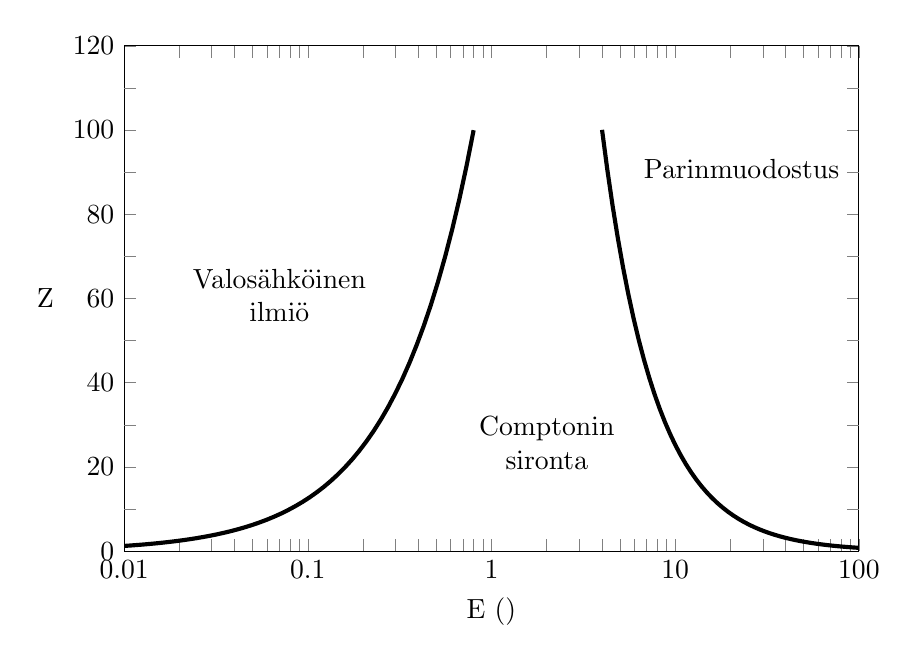
\begin{tikzpicture} %\cite{evans_atomic_1955}, sivu 712
    \begin{semilogxaxis}[
        width=.9\textwidth,
        height=8cm,
        xlabel={E (\unit{\mega\electronvolt})},
        ylabel={\rotatebox{-90}{Z}},
        xmin=0.01, xmax=100,
        ymin=0, ymax=120,
        xtick={0.01,0.1,1,10,100},
        ytick={0,20,40,60,80,100,120},
        grid=none,
        major grid style={line width=.2pt,draw=gray!50},
        minor tick style={draw=none},
        tick label style={
            /pgf/number format/fixed,
        },
        xticklabel={%
            \pgfkeys{/pgf/fpu=true}%
            \pgfmathparse{pow(10, \tick)}%
            \pgfmathprintnumber{\pgfmathresult}%
            \pgfkeys{/pgf/fpu=false}%
        },
        log basis x={10},
        extra x ticks={0.02, 0.03, 0.04, 0.05, 0.06, 0.07, 0.08, 0.09, 0.2, 0.3, 0.4, 0.5, 0.6, 0.7, 0.8, 0.9, 2, 3, 4, 5, 6, 7, 8, 9, 20, 30, 40, 50, 60, 70, 80, 90},
        extra x tick labels = {},
        extra y ticks={10,30,50,70,90,110},
        extra y tick labels = {},
        extra tick style={grid=none},
    ]
        \addplot[
            domain=0.01:0.8, 
            samples=50, 
            color=black,
            line width=1.5pt,
        ]
        {125*x};
        \addplot[
            domain=4:100, 
            samples=50, 
            color=black,
            line width=1.5pt,
        ]
        {800/x^(1.5)};
        \node at (axis cs:0.07,60) {\begin{tabular}{c} Valosähköinen \\ ilmiö \end{tabular}};
        \node at (axis cs:2,25) {\begin{tabular}{c} Comptonin \\ sironta \end{tabular}};
        \node at (axis cs:23,90) {\begin{tabular}{c} Parinmuodostus \end{tabular}};
    \end{semilogxaxis}
\end{tikzpicture}
    \caption{Hallitseva säteilyn ja aineen vuorovaikutuksen laji. Vaaka-akselilla on säteilyn energia ja pystyakselilla aineen atomin järjestysluku. Kuva on muokattu lähteestä \cite{evans_atomic_1955}.}
    \label{fig:vuorovaikutus}
\end{figure}

Valosähköisessä ilmiössä gammakvantti siirtää koko energiansa atomin elektronille, jolloin elektroni poistuu atomista. Valosähköinen ilmiö esiintyy yleensä pienillä gammakvantin energioilla ($<$\qty{0.5}{\mega\electronvolt}). Osa energiasta menee elektronin irrottamiseen atomista ja jäljelle jäävä energia muuttuu elektronin ja atomin kineettiseksi energiaksi.\cite{cherry_interaction_2012}

Comptonin sironnassa gammakvantti törmää atomissa olevaan heikosti sidottuun elektroniin luovuttaen osan energiastaan elektronille. Törmäyksen seurauksena elektroni irtoaa, mutta valosähköisestä ilmiöstä poiketen gammakvantti ei katoa. Gammakvantti jatkaa etenemistä pienemmällä energialla ja pidemmällä aallonpituudella. Comptonin sironta hallitsee energia-alueella \qtyrange{0.5}{3}{\mega\electronvolt}.\cite{cherry_interaction_2012}

Gammakvantti voi myös muuttua positroniksi ja elektroniksi törmätessään atomin ytimeen. Tämä vaatii gammakvantilta ainakin elektronin ja positronin yhteenlasketun lepomassan verran energiaa ekvivalenssiperiaatteen $E=mc^2$ mukaisesti, eli yli \qty{1.022}{\mega\electronvolt}. Kaavassa $E$ on energia, $m$ on massa ja $c$ on valonnopeus. Jäljelle jäävä energia jakautuu positronin ja elektronin kineettisiin energioihin liikemäärän säilymislain mukaisesti eli positroni ja elektroni etenevät vastakkaisiin suuntiin.\cite{cherry_interaction_2012}

Rayleighin sironnassa gammakvantin ja atomin voidaan ajatella törmäävän toisiinsa elastisesti. Verrattaessa Comptonin sironnassa irtoavaan elektroniin, atomin massa on hyvin suuri eli liike-energiasta siirtyy atomille vain hyvin pieni osa. Tästä johtuen Rayleighin sironnalla ei ole käytännön merkitystä isotooppilääketieteessä. Rayleighin sironta on myös merkittävää ainoastaan matalaenergisillä (alle \qty{50}{\kilo\electronvolt}) gammakvanteilla.\cite{cherry_interaction_2012}

Gammakuvantamisessa havaittava säteily on energialtaan \qtyrange{80}{500}{\kilo\electronvolt}. Tämän energia-alueen fotonit lävistävät ihmiskehon tehokkaasti, mutta ovat verrattain helposti pysäytettävissä detektorin tiheällä tuikeaineella ja säteilyltä voidaan suojautua esimerkiksi lyijyllä.\cite{cherry_gamma_2012}.

\subsection{Merkkiaineet}
Atomien välisten sidosten muodostumisen määrittää pitkälti elektronien sijanti. Koska radioaktiivinen hajoaminen tapahtuu atomin ytimessä, virittyneessä tilassa oleva ydin ei vaikuta atomin kemiallisiin sidoksiin. Vastaavasti kemialliset sidokset eivät vaikuta atomin radioaktiivisuuteen.\cite{cherry_modes_2012} Juuri tämä mahdollistaa radioisotooppien käytön isotooppilääketieteessä, kun radioaktiivinen yhdiste käyttäytyy biologisesti täsmälleen samoin kuin vakaa yhdiste. Käytännössä biologisesti vaikuttavasta molekyylistä, eli merkkiaineesta, korvataan jokin atomi sen radioaktiivisella isotoopilla tai hyvin samankaltaisesti käyttäytyvällä molekyylillä\cite{cherry_modes_2012, crisan_radiopharmaceuticals_2022}. Esimerkiksi glukoosilla on elintärkeä rooli ihmisen aineenvaihdunnassa. Korvaamalla glukoosin toinen hydroksyyliryhmä $\beta^{+}$-aktiivisella \ce{^{18}F}-atomilla saadaan fluorodeoksyglukoosi (FDG). FDG leviää elimistössä tavallisen glukoosin tavoin, joten havaitsemalla positronien annihilaatiotapahtumista syntyvät gammakvantit ihmiskehon ulkopuolelta voidaan arvioida glukoosin jakautumista kehossa.\cite{crisan_radiopharmaceuticals_2022}

Yksifotoniemissiotomografiassa yleisimmin käytetty isotooppi on metastabiili \ce{^{99m}Tc}, josta voidaan vastaavasti muodostaa eri tavalla vaikuttavia merkkiaineita. Teknetiumin etu verrattuna muihin radionuklideihin on sen kyky muodostaa erilaisia sidoksia. Siten teknetiumiin perustuvia merkkiaineita on verrattain helppoa kehittää eri tarkoituskohteisiin, kuten sydämen ja munuaisten toiminnan tutkimiseen.\cite{crisan_radiopharmaceuticals_2022}

\ce{^{99m}Tc}:n puoliintumisaika on \qty{6}{\hour} ja hajoamisessa syntyvän gammakvantin energia on noin \qty{141}{\kilo\electronvolt}.\cite{cherry_interaction_2012, cherry_single_2012, crisan_radiopharmaceuticals_2022, van_audenhaege_review_2015} Metastabiilin teknetiumin ominaisuudet tekevät siitä lähes optimaalisen gammakameralla havaitsemiseen. Tämän lisäksi, koska \ce{^{99m}Tc} muodostaa hajotessaan ainoastaan gammasäteilyä ja puoliintumisaika on suhteellisen lyhyt, myös kuvantamisen säteilyaltistus pysyy ajallisesti lyhyenä.\cite{cherry_modes_2012, crisan_radiopharmaceuticals_2022}

Muita yksifotoniemissiotomografiassa yleisesti käytettyjä radioisotooppeja ovat jodi-123, xenon-133, tallium-201 ja indium-111. Jodia käytetään yleensä aivojen dopamiinireseptorien toiminnan ja kaasumaista ksenonia puolestaan keuhkojen toiminnan kuvantamisessa. Talliumilla on sovelluskohteensa sydämen perfuusion kuvantamisessa, mutta sittemmin teknetium on pitkälti syrjäyttänyt sen käytön. Indiumiin pohjautuvilla merkkiaineilla kuvannetaan yleisesti syöpäkasvaimia. Indiumilla leimatuilla valkosoluilla voidaan myös selvittää tarkemmin elimistön tulehdustilaa.\cite{crisan_radiopharmaceuticals_2022}

\subsection{Gammakamera}
Yksifotoniemissiotomografiassa säteilyn havaitsemiseen perinteisesti käytetyn gammakameran rakenteen poikkileikkaus on esitetty \hyperref[fig:spect-detektori]{Kuvassa \ref*{fig:spect-detektori}}. Kamera koostuu valon elektroneiksi muuttavista valomonistinputkista, joiden päällä on levy säteilyn näkyväksi valoksi muuttavaa tuikeainetta. Näiden päällä on säteilyä valikoivasti läpäisevä kollimaattori.\cite{van_audenhaege_review_2015, cherry_gamma_2012}

\begin{figure}[H]
    \centering
    \captionsetup{width=.9\textwidth}
    \begin{tikzpicture}
    % Säteily
    \foreach \x in {-0.1, -0.06, ..., 0.14} {
        \draw[red] (3.5 + \x, 0) -- (3.5 - 2*4.5*\x, 5);
    }
    \node[right] at (8, 3) {Säteily};

    % Kollimaattori
    \foreach \x in {0,0.3,...,7}
        \fill (\x,0) rectangle (\x + 0.1,1);
    \node[right] at (8, 0.5) {Kollimaattori};

    % Tuikeaine
    \draw (0,0) rectangle (7,-1);
    \fill[pattern=north east lines] (0,0) rectangle (7,-1);
    \node[right] at (8, -0.5) {Tuikeaine};

    % Valomonistinputket
    \foreach \x in {0.5,1.5,...,6.5}{
        \fill[blue!40] 
        (\x-0.5,-1) --
        (\x+0.5,-1) --
        (\x+0.3,-1.5) --
        (\x+0.3,-3) --
        (\x-0.3,-3) --
        (\x-0.3,-1.5) --
        cycle;
    }
    \node[right] at (8, -2) {Valomonistinputket};
\end{tikzpicture}
    \caption{Yksifotoniemissiotomografiassa käytetyn gammakameran rakenteen poikkileikkaus. Kuvassa esitetyt gammakameran osat ovat ylhäältä alaspäin kollimaattori, joka päästää läpi vain tietystä suunnasta tulevan fotonin, tuikeaine, joka muuttaa fotonin näkyväksi valoksi sekä valomonistinputket, jotka muuttavat näkyvän valon elektroneiksi. Punaisilla viivoilla on havainnollistettu aluetta, jolta yksi kollimaattorin reikä kerää säteilyä detektorille.}
    \label{fig:spect-detektori}
\end{figure}

Tärkein gammakameran osa kuvan laadun kannalta on kollimaattori, joka sijaitsee säteilylähteen ja tuikeainekiteen välissä. Kollimaattorin tarkoituksena on päästää detektorille vain tietystä suunnasta tuleva säteily ja vaimentaa muista suunnista tuleva säteily, jotta hajoamistapahtuman alkuperä olisi mahdollista paikantaa tarkasti.\cite{cherry_gamma_2012, slomka_novel_2022}

Nämä toivotut ominaisuudet toteuttaa parhaiten raskaasta alkuaineesta valmistettu reikälevy, jossa reiät ovat olleet perinteisesti kuusikulmaisia tai pyöreitä.\cite{van_audenhaege_review_2015, cherry_gamma_2012} Uusimmissa laitteissa on yleistynyt neliön muotoisten reikien käyttö\cite{ljungberg_spectct_2018, slomka_novel_2022}. Mahdollisia materiaaleja reikien välille ovat muun muassa lyijy, wolframi, kulta, uraani ja platina\cite{van_audenhaege_review_2015}, mutta kustannusten vuoksi\cite{van_audenhaege_review_2015} kollimaattori on lähes aina valmistettu lyijystä tai wolframista.\cite{cherry_gamma_2012}

Koska kollimaattorin reikä ei todellisuudessa ole äärettömän pitkä tai äärettömän ohut, hajoamistapahtuman sijaintia ei ole mahdollista määrittää tarkasti. Tämä on perimmäinen syy siihen, miksi yksifotoniemissiotomografian kuvan laatu on merkittävästi huonompi kuin positroniemissiotomografian tai tietokonetomografian kaltaisissa kuvantamismenetelmissä, joissa ei käytetä kollimaattoria.\cite{cherry_gamma_2012} Gammakamera ei ole myöskään geometrialtaan optimaalinen, sillä alle \qty{0,1}{\percent} säteilystä havaitaan\cite{slomka_novel_2022}.
 
Yleisesti käytössä on neljänlaisia kollimaattoreita: suora kollimaattori (\textit{parallel-hole}), suppeneva (\textit{converging}) ja hajaantuva (\textit{diverging}) kollimaattori sekä yhden reiän kollimaattori (\textit{pinhole})\cite{cherry_gamma_2012, van_audenhaege_review_2015}.

\begin{figure}[H]
    \centering
    \captionsetup{width=.9\textwidth}
    \begin{subfigure}[t]{.4\textwidth}
        \resizebox{\linewidth}{!}{\begin{tikzpicture}
    % Kollimaattori
    \foreach \x in {-3.5, -3.2, ..., 3.5}
        \fill (\x,0) rectangle (\x + 0.1,1);

    % Tuikeaine
    \draw (-3.5, 0) rectangle (3.5, -1);
    \fill[pattern=north east lines] (-3.5, 0) rectangle (3.5, -1);
\end{tikzpicture}}
        \caption{}
    \end{subfigure}%
    \hspace{.1\textwidth}%
    \begin{subfigure}[t]{.4\textwidth}
        \resizebox{\linewidth}{!}{\begin{tikzpicture}
    % Kollimaattori
    \foreach \x in {-3.5, -3.2, ..., 3.5}{
        \fill[black]
            (\x, 0) --
            ({\x + 0.1}, 0) --
            ({0.8 * (\x + 0.1)}, 1) --
            ({0.8 * \x}, 1) --
            cycle;
    }

    % Tuikeaine
    \draw (-3.5, 0) rectangle (3.5, -1);
    \fill[pattern=north east lines] (-3.5, 0) rectangle (3.5, -1);
\end{tikzpicture}}
        \caption{}
    \end{subfigure}
    \begin{subfigure}[b]{.4\textwidth}
        \resizebox{\linewidth}{!}{\begin{tikzpicture}
    % Kollimaattori
    \foreach \x in {-3.5, -3.2, ..., 3.5}{
        \fill[black]
            (\x, 1) --
            ({\x + 0.1}, 1) --
            ({0.8 * (\x + 0.1)}, 0) --
            ({0.8 * \x}, 0) --
            cycle;
    }

    % Tuikeaine
    \draw ({0.8 * -3.5}, 0) rectangle ({0.8 * 3.5}, -1);
    \fill[pattern=north east lines] ({0.8 * -3.5}, 0) rectangle ({0.8 * 3.5}, -1);
\end{tikzpicture}}
        \caption{}
    \end{subfigure}%
    \hspace{.1\textwidth}%
    \begin{subfigure}[b]{.4\textwidth}
        \resizebox{\linewidth}{!}{\begin{tikzpicture}
    % Kollimaattori
    \fill[black]
        (-3.5, 0) --
        (-3.3, 0) --
        (-0.05, 2) --
        (-0.1, 2) --
        cycle;
    \fill[black]
        (3.5, 0) --
        (3.3, 0) --
        (0.05, 2) --
        (0.1, 2) --
        cycle;

    % Tuikeaine
    \draw (-3.5, 0) rectangle (3.5, -1);
    \fill[pattern=north east lines] (-3.5, 0) rectangle (3.5, -1);
\end{tikzpicture}}
        \caption{}
    \end{subfigure}
    \caption{Poikkileikkaus erilaisista kollimaattoreista. Mustien palkkien välit kuvaavat kollimaattorien reikiä ja osittain väritetty alue kuvaa tuikeainetta.}
    \label{fig:kollimaattorit}
\end{figure}

\hyperref[fig:kollimaattorit]{Kuvassa \ref*{fig:kollimaattorit}} on havainnollistettu eri tyyppisiä kollimaattoreita. Kuvan (a) kollimaattorissa reiät ovat suoria lieriöitä, kuvien (b) ja (c) kollimaattoreissa reiät muodostavat polttopisteen johonkin pisteeseen kollimaattorin ulkopuolelta ja kuvan (d) kollimaattorissa on vain yksi reikä.

Kuvantamisen kannalta huomioimisen arvoista on kollimaattorin mahdollinen suurennos tai pienennös. Kuvan (c) hajaantuvassa kollimaattorissa polttopiste on tuikeaineen takana, joten kuva pienenee. Vastaavasti kuvan (b) kollimaattorin polttopiste on kollimaattorin edessä, joten kuva suurenee. Kuvan (a) kollimaattorin polttopiste on käytännössä äärettömän kaukana, jolloin kuvan koko pysyy samana.\cite{cherry_gamma_2012, van_audenhaege_review_2015} Yksifotoniemissiotomografialaitteen suunnittelussa kollimaattorin tyyppi määrää sen, minkä kokoisia kohteita laitteella voidaan kuvantaa. Esimerkiksi detektorin pinta-alaa pienemmän kohteen, kuten aivojen, kuvantamiseen on optimaalista käyttää kuvan (b) kaltaista kollimaattoria. Vastaavasti kuvan (c) kollimaattoria voidaan käyttää detektoria suurempien kohteiden kuvantamiseen. Yhden reiän kollimaattorilla saadaan suhteellisen tarkkoja kuvia kilpirauhasen kaltaisista pienistä kohteista.\cite{van_audenhaege_review_2015, cherry_single_2012}

Kollimaattorin läpäisevä säteily pysähtyy tuikeaineeseen muodostaen näkyvää valoa. Ominaisuus löytyy esimerkiksi tietyistä yhdisteistä, joilla on säännöllinen hilarakenne. Näihin materiaaleihin lukeutuu muun muassa natriumjodidi, cesiumjodidi sekä tietyt ortosilikaatit ja polymeerit. Eri materiaalit eroavat toisistaan etenkin tiheydessä (eli säteilyn vaimenemisessa), syntyvän valon aallonpituudessa ja määrässä gammafotonia kohti, taitekertoimessa sekä valon välähdyksen kestossa.\cite{knoll_radiation_2010} Yleisin tuikeaine on natriumjodidi, johon on lisätty talliumia\cite{cherry_gamma_2012, cherry_single_2012, knoll_radiation_2010}. Natriumjodidin etuna ovat tehokas näkyvän valon tuotto ja edullisuus, mutta toisaalta valon välähdys kestää suhteellisen pitkään, mikä vaikeuttaa gammafotonien erottamista toisistaan\cite{knoll_radiation_2010}.

Tuikeainelevyn takana on säännöllisesti aseteltuja valomonistinputkia, joissa valokvantin energia irrottaa elektronin putken toisesta päästä. Putkessa on useita eri sähköisissä potentiaaleissa olevia elektrodeja, joista vuorotellen irtoaa yhä enemmän elektroneja. Valomonistinputken vahvistama signaali voidaan siirtää digitaalimuuntimelle ja tallentaa tietokoneelle.\cite{cherry_gamma_2012, knoll_radiation_2010} Koska valo etenee tuikeaineessa joka suuntaan, käytännössä aina valo havaitaan useammalla valomonistinputkella. Tällöin valokvantin tarkka sijainti voidaan laskea vertaamalla eri putkista havaittuja signaaleja. Yleensä tuikeaine jaetaan neliön muotoisiin pikseleihin, joihin tietyssä ajassa havaitut valokvantit paikannetaan\cite{cherry_gamma_2012, knoll_radiation_2010}.

\textcolor{red}{Tähän perinteisen gammakameran haitat}

Nykyaikaiset puolijohteisiin perustuvat säteilyilmaisimet muuttavat säteilyn energian suoraan sähköiseksi signaaliksi. Puolijohdemateriaaliin asetetaan ulkoinen jännite, joka muodostaa ionisaation tapahtuessa havaittavan jännitteen. Yleisimmät materiaalit ovat pii, germanium, kadmiumtelluridi (CdTe) sekä kadmiumsinkkitelluridi (CZT). Verrattuna perinteiseen ilmaisimeen, puolijohdeilmaisimet erottelevat paremmin fotonien energioita, tuottavat suuremman sähköisen signaalin fotonia kohti sekä ovat pienempiä. Toisaalta puolijohdeilmaisimet ovat herkkiä lämpötilan vaihteluille ja kohinalle, alttiita vaurioille säteilyaltistuksesta sekä verrattain kalliita.\cite{knoll_radiation_2010, slomka_novel_2022}

\textcolor{red}{Miksi puolijohdeilmaisimille on kysyntää?}